\documentclass[10pt]{article}
\usepackage{tikz}
\usepackage[margin=0cm]{geometry}
\pagestyle{empty}

\begin{document}

\vspace*{\fill}
\begin{center}
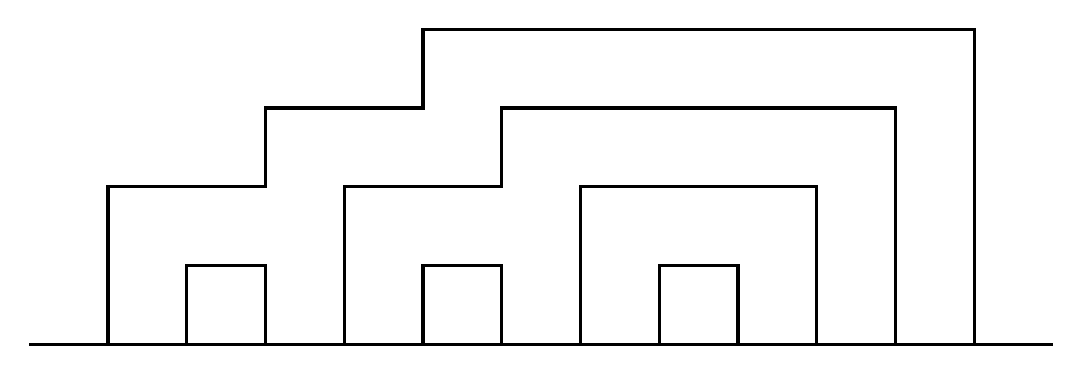
\begin{tikzpicture}[x=1.0cm, y=1.0cm, very thick]
\draw (-1,0) -- (12,0);
% Arch 1
    \draw (0,0) -- (0,2) -- (2,2) -- (2,3) -- (4,3) -- (4,4) -- (11,4) -- (11,0);
% Arch 2
    \draw (1,0) -- (1,1) -- (2,1) -- (2,0);
% Arch 3
    \draw (3,0) -- (3,2) -- (5,2) -- (5,3) -- (10,3) -- (10,0);
% Arch 4
    \draw (4,0) -- (4,1) -- (5,1) -- (5,0);
% Arch 5
    \draw (6,0) -- (6,2) -- (9,2) -- (9,0);
% Arch 6
    \draw (7,0) -- (7,1) -- (8,1) -- (8,0);
\end{tikzpicture}
\end{center}
\vspace*{\fill}

\end{document}
